\chapter{Good qLDPC Codes and LTC.}

The existence of good QLDPC codes and LTC were considered open problems for roughly two decades. Even though they seemed to be related only by containing the word "code" in their title, they were proven to exist by the same construction. They first appeared in \cite{Dinur} as good locally testable codes and not long after that in \cite{Pavel}, in which they also extended and derived the result to obtain the quantum code. Here, we follow the \cite{leverrier2022quantum} work, which simplifies the original proof and doesn't rely on any concept more complicated than what we already saw in the previous chapters. They also coined the term "Quantum Tanner Codes".


\section{Quantum Tanner Codes.}
Recall our insight that for a pair of LDPC codes to define a good CSS code, they must both be poor codes and have a constant distance. Therefore, we understand that any codeword in $C_{X}$ with small weight belongs to $C_{Z}^\perp$. To prove this, we will construct a proof such that if $x \in C_{X}$ and $|x|$ is small, then there is a small codeword $z \in C_{Z}^{\perp}$ such that $|x+z| < |x|$; by repeating this process recursively, it follows that $x\in C_{Z}^{\perp}$. To formulate this theorem, we will need to define more defintions.
  
 The next two definitions are concerned with the properties of the small code that will be set on the edges. Using them, one can characterize cases in which a local view can be reduced by subtracting a codeword from the dual code. 

\begin{definition}[$w$-Robustness] 
  \label{def:wrobust}
Let $C_0$ be a code of length $\Delta$ with minimum distance $\delta_0\Delta$. $C = \duC $ will be said to be $w$-robust if for any codeword $c \in C$ of weight less than $w$, it follows that $c$ can be decomposed into a sum of $c = t + s$ such that $t \in C_A \otimes \mathbb{F}^{B}$ and $s \in \mathbb{F}^A \otimes C_B$, where $s$ and $t$ are each supported on at most $\frac{w}{\delta_0\Delta}$ rows and columns. For convenience, we will denote by $B'$ ($A'$) the rows (columns) supporting $t$ ($s$) and use the notation $t \in C_A \otimes \mathbb{F}^{B'}$.
\end{definition}

\begin{figure}[H]
  \label{fig:wrobustf}
  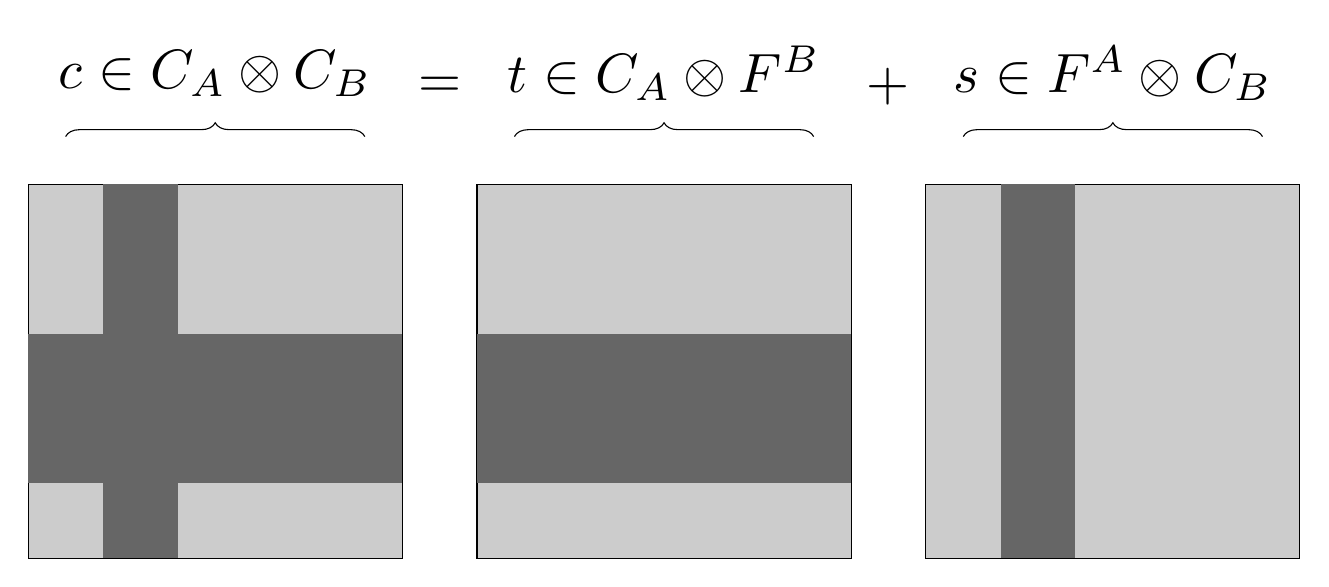
\begin{tikzpicture}[scale=0.95]

    \draw (5.5,6.3) node[scale=2]  { $=$ };
    \draw (11.5,6.3) node[scale=2]  { $+$ };

\draw [decorate,decoration={brace,amplitude=5pt,raise=4ex}] 
(0.5,5) -- (4.5,5) node[scale=2,midway,yshift=2em]{$c \in C_{A}\otimes C_{B}$};
        \filldraw [fill=white!80!black](0,0) rectangle (5,5);
       \fill [fill=gray!80!black] (1,0) rectangle (2,5);
        \fill [fill=gray!80!black] (0,1) rectangle (5,3);
\filldraw [fill=white!80!black](6,0) rectangle (11,5);
 \draw [decorate,decoration={brace,amplitude=5pt,raise=4ex}] 
 (6.5,5) -- (10.5,5) node[scale=2,midway,yshift=2em]{$t \in C_{A}\otimes \mathbb{F}^{B}$};
       \fill [fill=gray!80!black,draw opacity=0.5] (6,1) rectangle (11,3);
\filldraw [fill=white!80!black](12,0) rectangle (17,5);
  \draw [decorate,decoration={brace,amplitude=5pt,raise=4ex}] 
  (12.5,5) -- (16.5,5) node[scale=2,midway,yshift=2em]{$s \in \mathbb{F}^{A}\otimes C_{B}$};
     \fill [fill=gray!80!black,draw opacity=0.5] (13,0) rectangle (14,5);
            \end{tikzpicture}
            \caption{$w$-Robustness, Any low-weight codeword of the dual tensor code $c$ can be decomposed into a sum $t+s$, where $t$ is a collection of rows, each of which is a codeword in $C_A$, and similarly $s$ is a collection of columns, each of which is a codeword of $C_B$. }
\end{figure}



The definition we gave for $w$-Robustness is identical to the one stated by Zemor and Leverrier, but we also included the decomposition property in the definition. We refer the readers to the appendix section in \cite{leverrier2022quantum} for an existence proof by random construction. We mention that the random construction also gives the Gilbert-Varshamov bound.

\begin{definition}[$p$-Resistance to Puncturing.] Let $p,w$ be integers. We will say that the dual tensor code $C_{A} \otimes \mathbb{F} + \mathbb{F} \otimes C_{B}$ is $w$-robust with $p$-resistance to puncturing, if the code obtained by removing (puncturing) a subset of at most $p$ rows and columns is $w$-robust.   
\end{definition}

\begin{definition}[Quantum Tanner Code.]

%  Let $\Gamma$ be a group on $n$ verices. And let $A,B$ be a two generator set of $\Gamma$ such that if $a \in A$ ($B$) then also $a^{-1}\in A$ and that for any $g\in \Gamma,a \in A, b \in B$ it holds that $g \neq agb$ . Define the left right Cayley complex to be the graph $G = \left( \Gamma, E \right) $ obtain by taking the union of the two Cayley graphs generated by $A$ and $B$. So the vertices pair $u,v$ are set on square diaginal only if there are $a\in A$ and $b \in B$ such that $u = avb$. We can assume that $G$ is a bipartite graph (otherise just take $\Gamma^{\prime} = \Gamma \times \mathbb{Z}_{2}$ and define the product to be $a\left( u,\pm \right) = \left( au, \mp \right)$). 
%
%  Now divide the graph into postivie and negative vertices according their coloring $V_{-}$ and $V_{+}$. And define the positive graph to be $G^{+} = \left( V_{+}, E \right)$ and by $G^{-} = \left( V_{-}, E \right)$ the negative graph, when $E$denotes the sqaures, put it defrently their is an edge between $v$ and $u$ in $G^{+}$ if both vertices are positive and they are lay on the ends of square's diongal.
%
%  The quantum tanner code is a CSS code, such $C_{X}$ defined to be the classical tanner code $\mathcal{T}\left(G^{+}, \left(C_{A}^\perp\otimes C_{B}^{\perp}\right)^{\perp} \right)$ and $C_{Z}$ define as $\mathcal{T}\left(G^{-}, \left(C_{A}\otimes C_{B}\right)^{\perp} \right)$. Noice that in contrast to classical tanner code, in the quantum case it will be more convinent to think codewords as assiments set on the squaers and not on the edges.  
%
  Let $\Gamma$ be a group at size $n$. And let $A,B$ be a two generator set of $\Gamma$ such that if $a \in A$ ($B$) then also $a^{-1}\in A$ ($B^{-1}$) and that for any $g\in \Gamma, a \in A, b \in B$ it holds that $g \neq agb$. Define the left-right Cayley complex to be the graph $G = \left( \Gamma, E \right)$ obtained by taking the union of the two Cayley graphs generated by $A$ and $B$. So the vertices pair $u,v$ are set on a square diagonal only if there are $a\in A$ and $b \in B$ such that $u = avb$. We can assume that $G$ is a bipartite graph (otherwise just take $\Gamma^{\prime} = \Gamma \times \mathbb{Z}_{2}$ and define the product to be $a\left( u,\pm \right) = \left( au, \mp \right)$). 


Now divide the graph into positive and negative vertices according to their coloring $V_{-}$ and $V_{+}$. And define the positive graph to be $G^{+} = \left( V_{+}, E \right)$ and by $G^{-} = \left( V_{-}, E \right)$ the negative graph, where $E$ denotes the squares, put differently there is an edge between $v$ and $u$ in $G^{+}$ if both vertices are positive and they are laid on the ends of a square's diagonal.


The quantum Tanner code is a CSS code, such that $C_{X}$ is defined to be the classical Tanner code $\mathcal{T}\left(G^{+}, \left(C_{A}^\perp\otimes C_{B}^{\perp}\right)^{\perp} \right)$ and $C_{Z}$ is defined as $\mathcal{T}\left(G^{-}, \left(C_{A}\otimes C_{B}\right)^{\perp} \right)$. Note that in contrast to the classical Tanner code, in the quantum case it will be more convenient to think of codewords as assignments set on the squares and not on the edges.
\end{definition}
\begin{figure}[H]
            %\label{fig:square}
            \begin{center}
            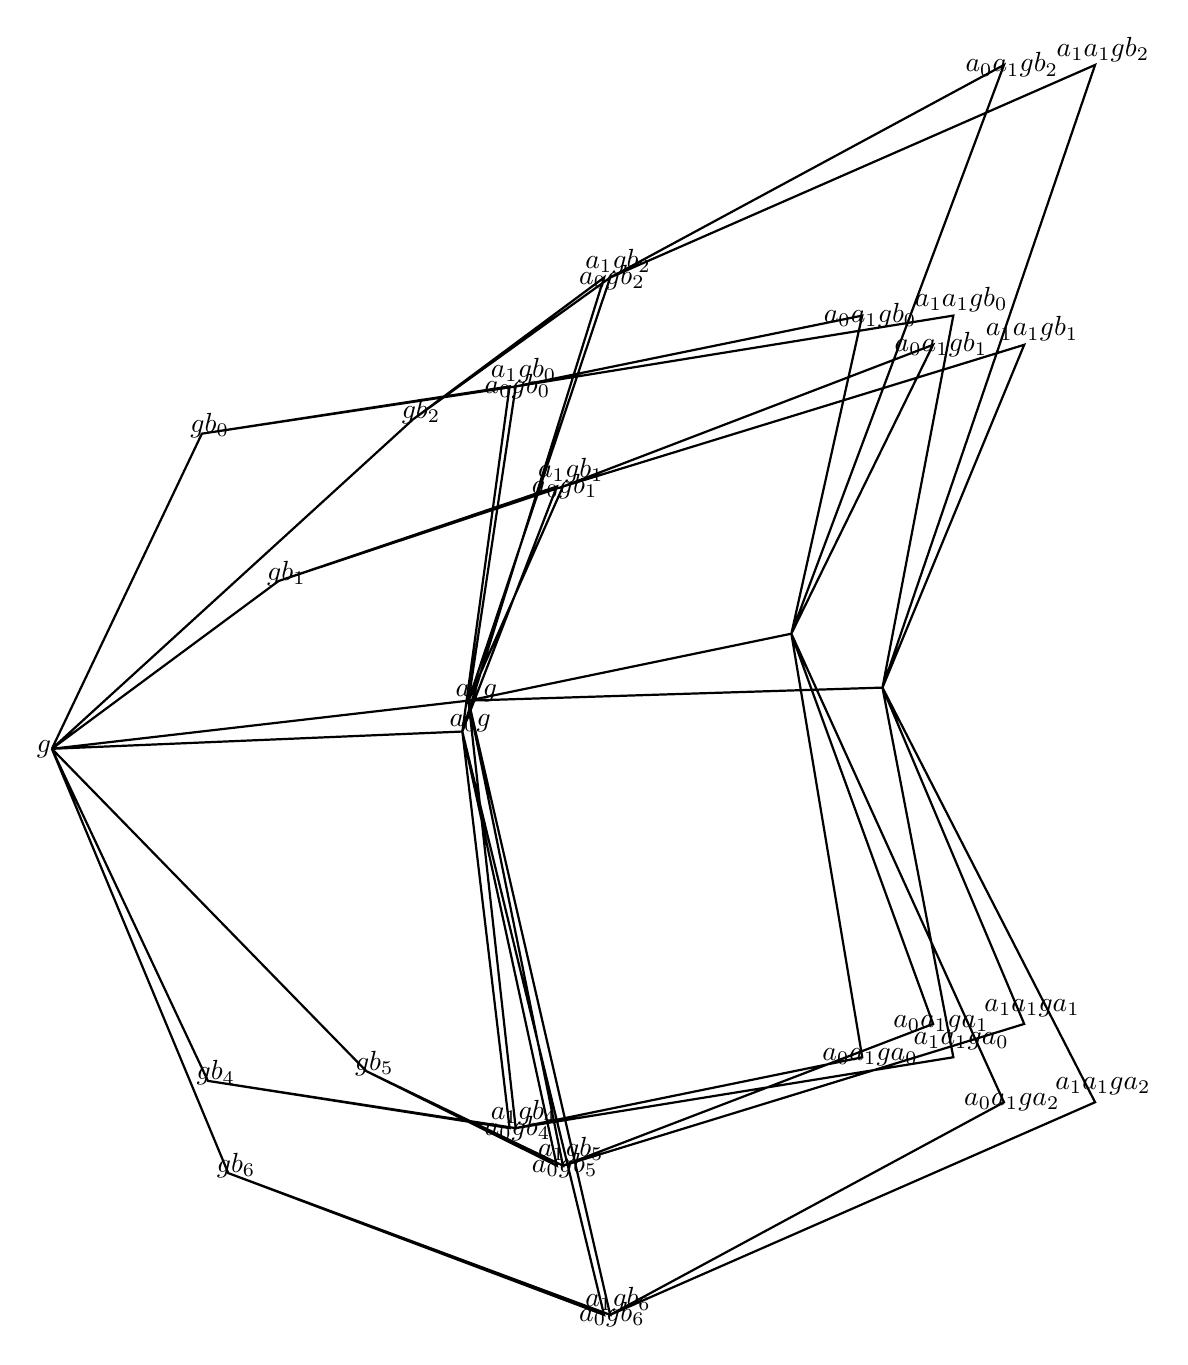
\begin{tikzpicture}
            \draw[thick](0,0)(0, 0) -- (1.9049911888377424,4.002079117547451) -- (5.81285084955138,4.602079117547451) -- (5.212850849551381,0.2192498173032679) -- (0, 0)
(0, 0) -- (2.879157898699928,2.130954290533681) -- (6.412850849551381,3.330954290533681) -- (5.212850849551381,0.2192498173032679) -- (0, 0)
(0, 0) -- (4.588270563356833,4.1850314105127575) -- (7.012850849551381,5.985031410512757) -- (5.212850849551381,0.2192498173032679) -- (0, 0)
(0, 0) -- (1.9049911888377424,4.002079117547451) -- (5.890590913653101,4.602079117547451) -- (5.2905909136531015,0.6119546131629411) -- (0, 0)
(0, 0) -- (2.879157898699928,2.130954290533681) -- (6.490590913653102,3.330954290533681) -- (5.2905909136531015,0.6119546131629411) -- (0, 0)
(0, 0) -- (4.588270563356833,4.1850314105127575) -- (7.090590913653101,5.985031410512757) -- (5.2905909136531015,0.6119546131629411) -- (0, 0)
(0, 0) -- (1.9818949186177792,-4.217396385887875) -- (5.81285084955138,-4.817396385887875) -- (5.212850849551381,0.2192498173032679) -- (0, 0)
(0, 0) -- (3.9944175473955323,-4.094159016671296) -- (6.412850849551381,-5.294159016671296) -- (5.212850849551381,0.2192498173032679) -- (0, 0)
(0, 0) -- (2.2401823432002748,-5.388664191428558) -- (7.012850849551381,-7.188664191428558) -- (5.212850849551381,0.2192498173032679) -- (0, 0)
(0, 0) -- (1.9818949186177792,-4.217396385887875) -- (5.890590913653101,-4.817396385887875) -- (5.2905909136531015,0.6119546131629411) -- (0, 0)
(0, 0) -- (3.9944175473955323,-4.094159016671296) -- (6.490590913653102,-5.294159016671296) -- (5.2905909136531015,0.6119546131629411) -- (0, 0)
(0, 0) -- (2.2401823432002748,-5.388664191428558) -- (7.090590913653101,-7.188664191428558) -- (5.2905909136531015,0.6119546131629411) -- (0, 0)
(5.2905909136531015, 0.6119546131629411) -- (5.890590913653101,4.602079117547451) -- (10.291575076901802,5.502079117547451) -- (9.391575076901802,1.4619219538089987) -- (5.2905909136531015, 0.6119546131629411)
(5.2905909136531015, 0.6119546131629411) -- (6.490590913653102,3.330954290533681) -- (11.191575076901803,5.130954290533681) -- (9.391575076901802,1.4619219538089987) -- (5.2905909136531015, 0.6119546131629411)
(5.2905909136531015, 0.6119546131629411) -- (7.090590913653101,5.985031410512757) -- (12.091575076901801,8.685031410512757) -- (9.391575076901802,1.4619219538089987) -- (5.2905909136531015, 0.6119546131629411)
(5.2905909136531015, 0.6119546131629411) -- (5.890590913653101,4.602079117547451) -- (11.4486392380322,5.502079117547451) -- (10.5486392380322,0.7771825477033486) -- (5.2905909136531015, 0.6119546131629411)
(5.2905909136531015, 0.6119546131629411) -- (6.490590913653102,3.330954290533681) -- (12.3486392380322,5.130954290533681) -- (10.5486392380322,0.7771825477033486) -- (5.2905909136531015, 0.6119546131629411)
(5.2905909136531015, 0.6119546131629411) -- (7.090590913653101,5.985031410512757) -- (13.248639238032201,8.685031410512757) -- (10.5486392380322,0.7771825477033486) -- (5.2905909136531015, 0.6119546131629411)
(5.2905909136531015, 0.6119546131629411) -- (5.890590913653101,-4.817396385887875) -- (10.291575076901802,-3.917396385887875) -- (9.391575076901802,1.4619219538089987) -- (5.2905909136531015, 0.6119546131629411)
(5.2905909136531015, 0.6119546131629411) -- (6.490590913653102,-5.294159016671296) -- (11.191575076901803,-3.494159016671296) -- (9.391575076901802,1.4619219538089987) -- (5.2905909136531015, 0.6119546131629411)
(5.2905909136531015, 0.6119546131629411) -- (7.090590913653101,-7.188664191428558) -- (12.091575076901801,-4.488664191428557) -- (9.391575076901802,1.4619219538089987) -- (5.2905909136531015, 0.6119546131629411)
(5.2905909136531015, 0.6119546131629411) -- (5.890590913653101,-4.817396385887875) -- (11.4486392380322,-3.917396385887875) -- (10.5486392380322,0.7771825477033486) -- (5.2905909136531015, 0.6119546131629411)
(5.2905909136531015, 0.6119546131629411) -- (6.490590913653102,-5.294159016671296) -- (12.3486392380322,-3.494159016671296) -- (10.5486392380322,0.7771825477033486) -- (5.2905909136531015, 0.6119546131629411)
(5.2905909136531015, 0.6119546131629411) -- (7.090590913653101,-7.188664191428558) -- (13.248639238032201,-4.488664191428557) -- (10.5486392380322,0.7771825477033486) -- (5.2905909136531015, 0.6119546131629411)
;
\node at (5.91285084955138,4.602079117547451) {$ a_{ 0  } gb_{ 0 } $};
\node at (6.512850849551381,3.330954290533681) {$ a_{ 0  } gb_{ 1 } $};
\node at (7.11285084955138,5.985031410512757) {$ a_{ 0  } gb_{ 2 } $};
\node at (5.990590913653101,4.802079117547451) {$ a_{ 1  } gb_{ 0 } $};
\node at (6.590590913653101,3.530954290533681) {$ a_{ 1  } gb_{ 1 } $};
\node at (7.190590913653101,6.1850314105127575) {$ a_{ 1  } gb_{ 2 } $};
\node at (5.91285084955138,-4.817396385887875) {$ a_{ 0  } gb_{ 4 } $};
\node at (6.512850849551381,-5.294159016671296) {$ a_{ 0  } gb_{ 5 } $};
\node at (7.11285084955138,-7.188664191428558) {$ a_{ 0  } gb_{ 6 } $};
\node at (5.990590913653101,-4.617396385887875) {$ a_{ 1  } gb_{ 4 } $};
\node at (6.590590913653101,-5.094159016671296) {$ a_{ 1  } gb_{ 5 } $};
\node at (7.190590913653101,-6.988664191428557) {$ a_{ 1  } gb_{ 6 } $};
\node at (10.391575076901802,5.502079117547451) {$ a_{ 0  } a_{ 1 }gb_{ 0 } $};
\node at (11.291575076901802,5.130954290533681) {$ a_{ 0  } a_{ 1 }gb_{ 1 } $};
\node at (12.1915750769018,8.685031410512757) {$ a_{ 0  } a_{ 1 }gb_{ 2 } $};
\node at (11.5486392380322,5.702079117547451) {$ a_{ 1  } a_{ 1 }gb_{ 0 } $};
\node at (12.4486392380322,5.330954290533681) {$ a_{ 1  } a_{ 1 }gb_{ 1 } $};
\node at (13.3486392380322,8.885031410512756) {$ a_{ 1  } a_{ 1 }gb_{ 2 } $};
\node at (10.391575076901802,-3.917396385887875) {$ a_{ 0  } a_{ 1 }ga_{ 0 } $};
\node at (11.291575076901802,-3.494159016671296) {$ a_{ 0  } a_{ 1 }ga_{ 1 } $};
\node at (12.1915750769018,-4.488664191428557) {$ a_{ 0  } a_{ 1 }ga_{ 2 } $};
\node at (11.5486392380322,-3.717396385887875) {$ a_{ 1  } a_{ 1 }ga_{ 0 } $};
\node at (12.4486392380322,-3.294159016671296) {$ a_{ 1  } a_{ 1 }ga_{ 1 } $};
\node at (13.3486392380322,-4.288664191428557) {$ a_{ 1  } a_{ 1 }ga_{ 2 } $};
\node at (-0.1,0) {$ g $};
\node at (5.31285084955138,0.3192498173032679) {$ a_{ 0 }g $};
\node at (5.390590913653101,0.7119546131629411) {$ a_{ 1 }g $};
\node at (2.0049911888377423,4.102079117547451) {$ gb_{ 0 } $};
\node at (2.979157898699928,2.230954290533681) {$ gb_{ 1 } $};
\node at (4.6882705633568325,4.285031410512757) {$ gb_{ 2 } $};
\node at (2.0818949186177793,-4.117396385887876) {$ gb_{ 4 } $};
\node at (4.094417547395532,-3.9941590166712957) {$ gb_{ 5 } $};
\node at (2.340182343200275,-5.288664191428558) {$ gb_{ 6 } $};          
\end{tikzpicture}
\end{center}

            \caption{Local environment of a square complex.}
            \label{fig:square}
           
            \end{figure}

Now we can state formally the theorem: 

\begin{theorem}
  For $\varepsilon \in \left( 0,\frac{1}{2} \right)$, $\gamma\in \left( \frac{1}{2} + \varepsilon, 1 \right)$, $\delta_{0}> 0$, large enough $\Delta$, and small codes $C_{A},C_{B}$ with distance at least $\delta_{0}\Delta$ if the dual tensor code of $C_{A},C_{B}$ is $w$-robust and $\Delta^{\gamma}$ resistance to puncturing, then there exists an infinite family of square complexes for which the Tanner code defined by the complexes and the dual tensor code such that any codeword with weigh less than $ \frac{\delta_{0}}{4\Delta^{3/2 + \varepsilon}} \cdot n \Delta^{2} $ is reducible \cref{ire}.
\end{theorem}


\begin{claim}
  The distance of the dual tensor code is at least $\delta\Delta$.
  \label{claim:duweight}
\end{claim}
\begin{proof}
By the robustness property, any codeword of the dual tensor code with a weight less than $\delta_{0}\Delta$ is supported on at most one row. Let $c$ be such a codeword and denote by $i$ the number of the non-trivial row. Fix a $c^{\prime} \in C_{A}^{\perp}$ such that the $i$th coordinate of  $c^{\prime}$ is non-zero and consider the multiplication of $c$ with the codewords of $C_{A}^\perp \otimes C_{B}^\perp$ of the following form:
  \begin{equation*}
    \begin{split}
      J = \left\{ c^{\prime} \otimes c_{b} : c_{b}\in C_{B}^{\perp} \right\} 
    \end{split}
  \end{equation*}
  So the $i$th row of any $x \in J$ is a codeword of $C_{B}^{\perp}$ and in total, collecting all the $i$th rows of codewords in $J$ sums up to all the code words in $C_{B}^{\perp}$. On the other hand, $c\cdot x = 0$ for all $x \in J$; that is, $c\cdot x = c_{i} \cdot c_{b} = 0$. Thus we obtain that $c_{i} \in C_{B}$ and therefore $|c_{i}| \ge \delta_{0}\Delta \Rightarrow |c| \ge \delta_{0}\Delta$, which is a contradiction.
\end{proof}

\begin{definition}
Let $S$ and $S_{-}$ denote the positive and negative vertices that support the codeword $c \in C_{X}$, respectively. Furthermore, let $S_e$ and $S_n$ denote the exceptional and normal vertices, respectively, where the weight of the local view for any vertex in $S_e$ is greater than $\Delta^{3/2 + \varepsilon}$, and $S_n$ is the complementary set of vertices. An edge in $G$ will be said to be heavy if it supports more than $\Delta\delta - \Delta^{\frac{1}{2} + \varepsilon}/\delta$ squares in $G$. Let $T \subset S_{-}$ denote the negative vertices connected to $S_{n}$ by at least one heavy edge. Additionally, let $T_s \subset T$ denote the vertices in $S_-$ that are surrounded by only normal vertices. Finally, for any pair of vertex subsets $A,B$ such that $A \subset V_{+}$ and $B \subset V_{-}$, let $d_{B\rightarrow A}$ denote the average number of heavy edges leaving $B$ and going to $A$.
\end{definition}
\begin{claim}
  \label{claim:epss}
  for any $\varepsilon \in \left( 0,1 \right)$ and large enough $\Delta$  it holds that $ |S| \le \Delta^{\varepsilon}|S_{-}| $ 
\end{claim}
\begin{proof}
  Suppose not, namely that $|S| > \Delta^{\varepsilon}|S_{-}|$, then $|x|/|S_{-}| > \Delta^{\varepsilon}|x|/|S| > \Delta^{\varepsilon} \cdot \delta_{0}\Delta $ But:  
\begin{equation*}
  \begin{split}
    \frac{|x|}{|S_{-}|} = \frac{\Theta \left(E(S_{-},S_{-}) \right)}{|S_{-}|} \le \Theta(\Delta^{2})\frac{|S_{-}|}{n}  + \Theta(\Delta)  \rightarrow_{n\rightarrow \infty} \Theta(\Delta)
  \end{split}
\end{equation*}
\end{proof}

\begin{claim}
  \label{claim:portion}
  At least $ 1- \Delta^{-\frac{\varepsilon}{4}}$ portion of the negative vertices adjoin to only normal vertices. 
\end{claim}
% Define the graph $G^{\star} = (V_{-}, E^{\star})$ such that $E^{\star} = E \cup \left\{ \left\{g, xyg \right\} x\neq y, \in A\cup B \right\}$ And notice that the assumption follows that  any 
\begin{proof}
  Suppose through contradiction that for $\Delta^{-p}$ portion of the negative vertices $v_{-}\in V_{-}$ have at least one ($\Delta^{\gamma}$) sibling in $S_{e}$. Therefore $ \Delta^{-p} |S_{-}| \le \Delta |S_{e}|$ combining with \cref{claim:epss} it follows that $|S| \le \Delta^{1+\varepsilon + p }|S_{e}|$ : 
  \begin{equation*}
    \begin{split}
      \Delta^{3/2 + \varepsilon} & \le \frac{E(S,S_{e})}{|S_{e}|} = \Theta\left( \Delta^{2} \right)\frac{|S|}{n} + \Theta\left( \Delta \right)\sqrt{ \frac{|S|}{|S_{e}|}  }\\ 
      & \le \Theta(\Delta^{2}) \frac{|S|}{n} + \Theta(\Delta) \Theta\left( \Delta^{\frac{1+\varepsilon + p}{2}} \right)  
    \end{split}
  \end{equation*} 
  Thus we obtain contradiction for any $p < \varepsilon/2$. In particular for $p = \varepsilon/4$ we obtain that at least $1 - \Delta^{-\varepsilon/4}$ portion of the negative vertices are surounded by only normal vertices. 
 \end{proof}

 % \begin{claim}
%   Any $x \in \duC$ such that $|x| \le w$, and denote by $A^{\prime},B^{\prime}$ the rows and cols support $x$. Then $x$ can decompise into a sum of $x = t + s$ such that $t \in C_{A}\otimes \mathbb{F}^{B^\prime}$ and $s \in  \mathbb{F}^{A^\prime} \otimes  C_{B}$. 
% \end{claim}
% \begin{proof}
%   By induction on the number of raws supported $x$. Denote $x$ by 
%
%   \begin{equation*}
%     \begin{split}
%       x & = \sum_{i, c_{a}}{ c_{a} \otimes e_{i}  } + \sum_{i, c_{b} }{ e_{i} \otimes c_{b}} \\
%       & =  c_{a^{\prime}} \otimes e_{\tau} + \sum_{i / \tau, c_{a}}{ c_{a} \otimes e_{i}  } + \sum_{i, c_{b} }{ e_{i} \otimes c_{b}} \\
%      \end{split}
%   \end{equation*} 
%   
%   Now, if $c_{a^{\prime}} \otimes e_{\tau}$ decrese the summation weight then it must holds that $x$  
%
%    \begin{equation*}
%     \begin{split}
%       & =  c_{a^{\prime}} \otimes e_{\tau} + t^{\prime} + s^{\prime} = \overbrace{\left( c_{a^{\prime}} \otimes e_{\tau} + t^{\prime} \right) }^{ C_{A} \otimes \mathbb{F}^{B^{\prime}}}+ s^{\prime}
%     \end{split}
%   \end{equation*}
% \end{proof}
% 
 \begin{claim}  
   \label{claim:close}
   Let $x$ be a codeword of $\duC$ and $\xi < w$ such that $d(x, \mathbb{F}^{A} \otimes C_{B}) + d(x, C_{A}\otimes\mathbb{F}^{B}) \le \xi $ . Then $d(x, C_{A} \otimes C_{B}) < 3\xi $. 
 \end{claim} 
 \begin{proof}
Denote by $R$ the closest codeword of $C_{A}\otimes\mathbb{F}^{B}$ to $x$. Similarly, denote by $C$ the closest codeword of $\mathbb{F}^{A} \otimes C_{B}$ to $x$. Notice that $C + R \in \duC$. In addition, the weight of $C+R$ is bounded by:
   \begin{equation*}
     \begin{split}
       |R + C| &=  |x + \left(x + R\right) + x + \left( x + C\right)| \\
       & \le |\left(x + R\right)|+ |\left( x + C\right)| \le d\left( x ,   C_{A}\otimes\mathbb{F}^{B} \right) +  d\left( x ,   \mathbb{F}^{A} \otimes C_{B} \right) \\ 
       & \le w
     \end{split}
   \end{equation*}
   Therefore, by the robustness property, there are $r \in C_{A}\otimes\mathbb{F}^{B}$ and $c \in \mathbb{F}^{A} \otimes C_{B} $ such that $ R + C  = r + c$. And $r,c$ are supported on at most $|R+C|/\delta\Delta$ rows and columns. (Here $r$ and $c$ play the role of $s,t$ in \cref{def:wrobust}.)  

   Now observe that on one hand $C + c = R + r$, and on the other hand $ C + c \in \mathbb{F}^{A} \otimes C_{B} $ and $R+r \in C_{A}\otimes\mathbb{F}^{B}$. Therefore, $C+c \in C_{A}\otimes\mathbb{F}^{B} \cap \mathbb{F}^{A} \otimes C_{B}$. Namely, $C +c \in C_{A} \otimes C_{B}$. Thus we have:  
   
   \begin{equation*}
     \begin{split}
       d\left(x, C_{A}\otimes C_{B}\right) & \le d\left(x, C\right) + d\left(C, C_{A}\otimes C_{B} \right) \\
       &\le \xi + |c|
     \end{split}
   \end{equation*}
   And in the same way we obtain also that $d\left( x, C_{A} \otimes C_{B} \right) \le \xi + |r|$. Since $c,r$ are supported on at most $|R+C|/\delta\Delta$ rows and columns, the weight of the string obtained by joining a single row of $r$ with $c$ grows by at least $\delta\Delta - |R+C|/\delta\Delta > 0$. Therefore, $|c| < |c + r| = |R + C|$. Thus, in total, $d\left( x, C_{A} \otimes C_{B} \right) \le 3\xi$.
 \end{proof}

\begin{claim}
  \label{claim:closeto}
  Suppose that $v \in T_{s}$, Namely $v$ is surounded by only normal vertices. Then:
  \begin{equation*}
    \begin{split}
      d\left( c_{v}, C_{A}\otimes C_{B}\right) < \Theta\left( \Delta^{3/2+\varepsilon} \right)
    \end{split}
  \end{equation*} 
 \end{claim}
\begin{proof}
  By being surrounded only by normal vertices any row in the local view of $v$ is codeword of $C_{A}$ plus at most $\Delta^{3/2 + \varepsilon}/\Delta = \Delta^{\frac{1}{2}+\varepsilon}$ faults. So correcting the rows require flipping at most $\Delta \cdot \Delta^{\frac{1}{2} + \varepsilon}$ bits in total.  Thus $d\left(c_{v}, C_{A}\otimes \mathbb{F}^{B}\right) < \Delta^{3/2 + \varepsilon}$. In same way we obtain that $d\left(c_{v},  \mathbb{F}^{A} \otimes C_{B}\right) < \Delta^{3/2 + \varepsilon}$. Noitce that, in parituclar, $d(c_{v}, \duC) \le \Delta^{3/2 + \varepsilon}$.

  Denote by $y$ the closest codeword of $\duC$ to $c_{v}$. And observes that the distance between $y$ to either $C_{A} \otimes \mathbb{F}^{B}$ or $\mathbb{F}^{A}\otimes C_{B}$ is at most $2 \cdot \Delta^{3/2 + \varepsilon}$. To see it consider the decoding: 
  \begin{equation*}
    \begin{split}
  y \rightarrow x \rightarrow C_{A} \otimes \mathbb{F}^{B}   
    \end{split}
  \end{equation*}
  
  Therefore form \cref{claim:close} it follows that $d\left(y, C_{A} \otimes C_{B}\right) < 3 \xi $, So $d\left(x, C_{A} \otimes C_{B}\right) < \Delta^{3/2 + \varepsilon} +  3 \xi $.
     \end{proof}
   
   
 
 \begin{claim}[The Technical Lemma]  
   \label{cliam:tech} Let $A \subset S$ and $B \subset S_{-}$ subsets of the positive and the negetive vertices support $x$, and $\alpha \le \Delta^{2},\beta \le \Delta$ their minimal degrees in $G, G$. Assume the following conditions hold:
   \begin{enumerate}
     \item $\beta = \frac{\delta}{4 \sqrt{\Delta}}\alpha + \Theta\left(  \right)$
     \item $B$ defined to be all the vertices connected to $\bar{A}$ by at least one heavy edge.
     \item Any vertex in $\bar{A}$ has at least one heavy edge. 
   \end{enumerate}
   Then: $d_{B\rightarrow \bar{A}} = \Omega\left( \Delta \right)$.  
 \end{claim}

 \begin{proof}
   By the given $|S| \le \frac{2|x|}{\delta\Delta} \le \zeta\frac{2n\Delta}{\delta}$ we have that $|S|/n \le \zeta\cdot \frac{2\Delta}{\delta}$.
   %Let $A \subset S$ and $B \subset S_{-}$ subsets of the positive and the negetive vertices support $x$, and $\alpha \le \Delta^{2},\beta \le \Delta$ their minimal degrees in $G, G$.
   Then by the Mixing Expander Lemma we have that:   
   \begin{equation*}
     \begin{split}
       \alpha |A| & \le |E(A,S)| \le \frac{\Delta^{2}}{n}|A||S| + 4 \Delta \sqrt{|A||S|} \le |A| \cdot \zeta \frac{2\Delta^{3}}{\delta} +  4 \Delta \sqrt{|A||S|}\\ 
       & \Rightarrow \sqrt{|A|}\left(\alpha-\zeta \frac{2\Delta^{3}}{\delta}  \right) \le 4\Delta\sqrt{|S|} \\
       & \Rightarrow |A| \le \left( \alpha -  \zeta \frac{2\Delta^{3}}{\delta}  \right)^{-2} \cdot 16\Delta^{2}|S|
     \end{split}
   \end{equation*}
   And by repetting the same calculation but consider $B$ in the $G$ graph we obtain: 
\begin{equation*}
     \begin{split}
       \Rightarrow  |B| \le & \left( \beta -  \zeta \frac{4 \cdot 2\Delta^{2} }{\delta}  \right)^{-2} \cdot 16\Delta|S|\\
       \Rightarrow  |B| \le & \left( \frac{\delta}{\sqrt{\Delta}}\alpha   -  \zeta \frac{4 \cdot 2\Delta^{2} }{\delta}  \right)^{-2} \cdot 16\Delta|S|\\
       = & \frac{\Delta}{\delta^{2}} \left(  \alpha -  4\cdot 2\zeta \frac{\Delta^{2\frac{1}{2}}}{\delta^{2}}   \right)^{-2} \cdot 16\Delta|S| 
     \end{split}
   \end{equation*}
   And for large enugh $\Delta$ the above is bounded by:
   \begin{equation*}
     \begin{split}
     \left(  \alpha -  4\cdot 2\zeta \frac{\Delta^{2\frac{1}{2}}}{\delta^{2}}   \right) \ge \left( \alpha -  \zeta \frac{2\Delta^{3}}{\delta}  \right) \Rightarrow |B|  \le  & \frac{1}{\delta^{2}} \left( \alpha -  \zeta \frac{2\Delta^{3}}{\delta}  \right)^{-2} \cdot 16\Delta^{2}|S| 
     \end{split}
   \end{equation*}
   Now, choose $\zeta$ such $\left( \alpha -  \zeta \frac{2\Delta^{3}}{\delta}  \right) \ge 16^{\frac{1}{2}} \cdot 100 \Delta^{1\frac{1}{2}}$ yields that: $|A| \le 10^{-4}\Delta^{-1} |S| \Rightarrow $$ |\bar{A}| \ge \left( 1 - 10^{-4} \Delta^{-1}\right)|S|$, And $|B| \le 10^{-4} \frac{|S|}{16 \delta^{2}\Delta}$. Conditions (2) and (3) garunte that any vertex in $\bar{A}$ is connected to at least on vertex of $B$. And therfore, $B$ covers $\bar{A}$, that is, $ d_{B\rightarrow\bar{A}}\cdot |B| \ge \bar{A}$, Hence:

   \begin{equation*}
     \begin{split}
       d_{B\rightarrow \bar{A}}  \ge \frac{|\bar{A}|}{|B|} \ge \left( 1 - 10^{-4}\Delta^{-1}  \right) 10^{4} \cdot \delta^{2}\Delta  = \Theta\left( \Delta \right)
     \end{split}
   \end{equation*}
 \end{proof}
 
 \begin{claim}
   \label{claim:satis}
   $S_{e}$ and $T$ satisfies the requrirments of \cref{cliam:tech} with $A = S_{e}$, $B = T$, $\alpha = \Delta^{3/2 + \varepsilon}$ and $\beta = \Delta\delta + \Delta^{\frac{1}{2} + \varepsilon}$. That is, the average of havey edges form $T$ to $S_{n}$ is $\Theta\left( \Delta \right)$. 
 \end{claim}

 \begin{proof}
   Conditions (1) and (2) holds by definition of $S_{e},T$ for values $\alpha = \Delta^{3/2 + \varepsilon}$ and $\beta = \Delta\delta - \Delta^{\frac{1}{2}+\varepsilon}/\delta$. It left to show that any normal vertex has at least on heaviy edge. By \cref{claim:duweight} any normal vertex $v$ has weight at least $\Delta\delta$, yet by robustness there are $t,s \in C_{A}\otimes \mathbb{F}^{B}, \mathbb{F}^{B}\otimes  C_{B}$ such that $t+s = c_{v}$. Assume that that any row of $c_{v}$ has weight less than $\Delta\delta - \Delta^{\frac{1}{2}+\varepsilon}/\delta$. Pick an arbitery row, and denote it by $\tau$, Now observes that by the fact that $c_{v}$ has support on at most $\Delta^{\frac{1}{2}+\varepsilon}/\delta$ columns, then $\tau$ is at distance at most $\Delta^{\frac{1}{2}+\varepsilon}/\delta$ from $C_{A}$. But, by assumption, $|\tau| < \delta\Delta -\Delta^{\frac{1}{2}+\varepsilon}/\delta$ and therefore the closet codeword to $\tau$ in $C_{A}$ has weight less than  $\delta\Delta$ in contradiction to the fact that the distance of $C_{A}$ is at least $\delta\Delta$.  

Conditions (1) and (2) hold by definition of $S_e,T$ for values $\alpha = \Delta^{3/2 + \varepsilon}$ and $\beta = \Delta\delta - \Delta^{\frac{1}{2}+\varepsilon}/\delta$. It remains to show that any normal vertex has at least one heavy edge. By robustness there are $t,s \in C_{A}\otimes \mathbb{F}^{B}, \mathbb{F}^{B}\otimes  C_{B}$ such that $t+s = c_{v}$. Assume that any row of $c_{v}$ has weight less than $\Delta\delta - \Delta^{\frac{1}{2}+\varepsilon}/\delta$. Pick an arbitrary row, and denote it by $\tau$. Now observe that by the fact that $c_{v}$ has support on at most $\Delta^{\frac{1}{2}+\varepsilon}/\delta$ columns, then $\tau$ is at a distance of at most $\Delta^{\frac{1}{2}+\varepsilon}/\delta$ from $C_{A}$. But, by assumption, $|\tau| < \delta\Delta -\Delta^{\frac{1}{2}+\varepsilon}/\delta$ and therefore the closest codeword to $\tau$ in $C_{A}$ has weight less than $\delta\Delta$, in contradiction to the fact that the distance of $C_{A}$ is at least $\delta\Delta$.
 \end{proof}

\begin{claim}
  \label{claim:linear}
  There is a normal-surounded vertex in $v \in T_{s}$ in weight at least $\Theta\left(\Delta^{2}\right)$.   
 \end{claim}
 \begin{proof}
   We know from \cref{claim:satis} that $d_{T\rightarrow S_{n} }$ is linear in $\Delta$. Morever \cref{claim:portion} tell us that most of the vertices in $S_{-}$ are surrounded only by normal vertices. Denote by $\expp{ d(v) | v \in T_{s} }$ the expected degree of heavy edges connected to vertex in $T_{s}$. Using the conditional expection formula we get:
  
   \begin{equation*}
     \begin{split}
       d_{T \rightarrow S_{n}} &= \expp{ d(v) | v \in T_{s} } \prb{ v \in T_{s}} + \expp{d\left( v \right) | v \in T / T_{s}} \prb{ v \in T / T_{s}} \\
       & \le \expp{ d(v) | v \in T_{s} } \prb{ v \in T_{s}} + \expp{d\left( v \right) | v \in T / T_{s}} \prb{ v \in S_{-} / T_{s}} \\
       & \le \expp{ d(v) | v \in T_{s} } \cdot 1   + \Delta \cdot  \Delta^{-\varepsilon/4} \\
       & \Rightarrow  \expp{ d(v) | v \in T_{s} } \ge d_{T \rightarrow S_{n}} - \Delta^{\frac{3}{4} \varepsilon} = \Theta\left( \Delta \right) 
     \end{split}
   \end{equation*}
   Therefore there is at least a single vertex in $T_{s}$ connected to $\Theta\left( \Delta \right)$ havey edges. Combining the fact that edge is heavy edge if there are at least $\Delta\delta - \Delta^{\frac{1}{2} + \varepsilon}$ non trival bits on it's squares we get the desired.  
 \end{proof}

 We are about to finish the proof of the theorem. Combining \cref{claim:linear} and \cref{claim:closeto} we obtain the the existnes of a negative vertex which is both at distance $\Theta\left(\Delta^{3/2 + \varepsilon}\right)$ form $C_{A}\otimes C_{B}$ and weight at least $\Theta\left( \Delta^{2} \right)$. Denote by $v \in T_{s}$ that vertex, by $c_{v}$ it's local view and by $y \in C_{A}\otimes C_{B}$ the closest codeword to $c_{v}$. Subtructing $y$ from $c_{v}$ yilds: 
 
 \begin{equation*}
   \begin{split}
     \left|   c_{v} + y   \right| &= d\left( c_{v}, y  \right) = \Theta\left( \Delta^{3/2 + \varepsilon} \right) < \left|   c_{v}   \right|     \\
     \Rightarrow & | c + y| < |c| 
   \end{split}
 \end{equation*}

 \section{LTC.} 
As exactly as in the polynomial code case, we will prove that a code is locally testable by presenting a decoder that can correct small errors and reject errors greater than a linear threshold. But before that, let us define the LTC code.

\begin{definition}
Consider the Tanner code defined on the square complex above, but instead of taking the dual tensor as the local code, we take the product code: $\mathcal{T} \left(G^{+}, C_{A} \otimes C_{B} \right)$.
\end{definition}
Now, let us define the disagreement code, which we can conceptually think of as the strings obtained by an attempt to decode by local correction. That is, any vertex chooses the closest codeword to its local view and the summation of the suggestions is the disagreement. Notice that if the initial assignment was a valid codeword then each of the vertices suggest the codeword it sees on its local view. Hence, for any edge will suggest exactly the same bit and the summation on the edge will be equal to zero. Because it is true for all the edges, the total string obtained will be the zero codeword. Nevertheless, any assignment on an edge which equals $1$ points to a disagreement between the vertices at the edge's ends.
\begin{definition}[The Disagreement Code] Given a Tanner code $C = \Tann$, define the code $C_{\oplus}$ to contain all the words equal to the formal summation $ \sum_{v \in V\left( G \right)} {c_{v} }$ when $c_{v}$ is an assignment of a codeword $ c_{v} \in C_0 $  on the edges of the vertex $ v \in V\left( G \right)$.
  We call to such code the \textbf{disagreement code} of $C$, as edges are set to 1 only if their connected vertices contribute to the summation codewords that are different on the corresponding bit to that edge. In addition, we will call to any contribute $c_v$, the \textbf{suggestion} of $v$. And notice that by linearity, each vertex suggests, at most, a single suggestion.   

  Finally, given a bits assessment $x \in \mathbb{F}_{2}^{E}$ over the edges of $G$, we will denote by $x^{\oplus} \in C_{\oplus} $ the codeword which obtained by summing up suggestions set such each vertex suggests the closet codeword to his local view. Namely, for each $v \in V$ define:   
  \begin{equation*}
    \begin{split}
      c_{v} & \leftarrow \arg_{ \tilde{c} \in C_{0}} \min{ d( x|_{v} , \tilde{c} ) } \ \ \forall v\in V   \\
      x^{\oplus} & \leftarrow \sum_{v \in V}{c_{v}} 
    \end{split}
  \end{equation*}
  We will think about $x^{\oplus}$ as the disagreement between the vertices over $x$. 

\end{definition}

\begin{definition} Let $C = \Tann$. We say that $x \in C_{\oplus}$ is \textbf{reducible} if there exists a vertex $v$ and a small codeword $c_v$, for which, adding the assignment of $c_v$ over the $v$'s edges to $x$ decreases the weight. Namely, $|x + c_{v}| < |x|$. If $x \in C_{\oplus}$ is not a reducible codeword then we say that $x$ is \textbf{irreducible} \label{ire}. \end{definition}

The following lemma states that the disagreement is invariant when adding codewords, resulting in any decoder that can correct errors occurring to the trivial codeword by taking the derived disagreement as input being able to correct the same errors when they occur to any codeword.

\begin{lemma}[Linearity of The Disagreement] \label{lemma:lin} Consider the code $C = \Tann$. Let $ x \in \mathbb{F}_{2}^{E}$ then for any $ y \in C$ it holds that: 
  \begin{equation*}
    \begin{split}
      \left( x + y  \right)^{\oplus} = \left( x  \right)^{\oplus} 
    \end{split}
  \end{equation*}
\end{lemma}
  \begin{proof} Having that $y \in C$ followes $y|_v \in C_{0}$ and therefore 


    \begin{equation*}
      \begin{split}
        \arg_{ \tilde{c} \in C_{0}} \min{ d( z  , \tilde{c} ) } = y|_{v} + \arg_{ \tilde{c} \in C_{0}} \min{ d( z, \tilde{c} + y|_{v} ) } 
      \end{split}
    \end{equation*}
     Hence the suggestion made by vertrx $v$ is: 
  \begin{equation*}
    \begin{split}
      c_{v}\leftarrow &  \arg_{ \tilde{c} \in C_{0}} \min{ d( (x+y)|_{v}  , \tilde{c} ) } \\
      \leftarrow &  y|_{v} +  \arg_{ \tilde{c} \in C_{0}} \min{ d( (x+y)|_{v}  , \tilde{c} + y|_{v} ) } \\
      \leftarrow &  y|_{v} +  \arg_{ \tilde{c} \in C_{0}} \min{ d( x|_{v} , \tilde{c} ) } 
    \end{split}
  \end{equation*}
  It follows that: 

  \begin{equation*}
    \begin{split}
      \left( x + y \right)^{\oplus} =& \sum_{v\in V}{c_{v}} = \sum_{v \in V}{y|_{v}} + \sum_{v\in V}{ \arg_{ \tilde{c} \in C_{0}} \min{ d( x|_{v} , \tilde{c} ) } } \\ 
      =& y^{\oplus} + x^{\oplus} = x^{\oplus}
    \end{split}
  \end{equation*}
  When the last transition follows immediately by the fact that $y \in C$ and therefore any pair of connected vertices contribute the same value for their associated edge \end{proof}
%
%  \begin{definition} Let $C = \Tann$. We say that $x \in C_{\oplus}$ is \textbf{reducable} if there exists a vertex $v$ and a small codeword $c_v$, for which, adding the assignment of $c_v$ over the $v$'s edges to $x$ decreases the weight. Namely, $|x + c_{v}| < |x|$. If $x \in C_{\oplus}$ is not a reducable codeword then we say that $x$ is \textbf{ireducable} \label{ire}. \end{definition}
%
%


\section{Decoding and Testing}
  For completeness, we show exactly how Theorem 1 implies testability. The following section repeats Leiverar's and Zemor's proof \cite{leverrier2022quantum}. Consider a binary string $x$ that is not a codeword. The main idea is the observation that the number of bits filliped by (any) decoder, while decoding $x$, bounds the distance $d\left( x, C \right)$ from above. In addition, the number of positive checks in the first iteration is exactly the number of violated restrictions.
%\begin{figure*}[h]
%\begin{adjustbox}{width=\textwidth}
  \begin{definition}Let $L = \{L_{i}\}^{2|E|}_{0}$  be a series of $2|E|$. Such that for each vertex $ v \in V$ $\sum_{ e = \{u,v\} }{ L_{e_v} } \in C_{0}$. We will call $L$ a \textit{Potential list} and refer to the $e_{v}$'the element of $L$ as a suggestion made by the vertex $v \in V$ for the edge $e \in E$. Sometimes we will use the notation $L_{v}$ to denote all the $L$'s coordinates of the form $ L_{e_{v}} \forall e \in \text{Support} \left( v \right) $. Define the \textit{Force} of $L$ to be the following sum $  F\left( L \right) = \sum_{e = \{v,u\} \in E }{ \left(L_{e_v} + L_{e_u}\right) }$ and notice that $ F\left( L \right) \in C_{\oplus}$. And define the \textit{state} $S(L) \subset \mathbb{F}^{|E|}_{2}$ of $L$ as the vector obtained by choosing an arbitrary value from $ \{ L_{e_v}, L_{e_u} \}$ for each edge $e \in E$.  
  \end{definition}
  \begin{claim} \label{claim:pot} Let $L$ be the Potential list. If $F(L)=0$ then $S(L)\in C$. \end{claim}
  \begin{proof} Denote by $\phi\left( e \right) \subset \{ L_{e_v}, L_{e_u} \}$ the value which was chosen to $e = \{v,u\} \in E$. By $F\left(L\right) = 0$ , it follows that $ L_{e_v} + L_{e_u} = 0 \Rightarrow L_{e_v} = L_{e_u} = \phi\left( e \right) $ for any $e \in E$. Hence for every $v\in V$ we have that $ S\left( L \right)|_{v} = \sum_{u \sim v}{ \phi\left( \{v,u\} \right) } =  \sum_{u \sim v}{ L_{e_v }} \in C_{0}$ $ \Rightarrow S\left( L \right) \in C$   
  \end{proof}
  The decoding goes as follows. First, each vertex suggests the closet $C_{0}$'s codeword to his local view. Those suggestions define a Potential list, denote it by $L$, then if $F\left( L \right) <\tau$, by Theorem 1, one could find a suggestion of vertex $v$ and a codeword $c_v$ such that updating the value of $L_{v} \leftarrow L_{v} + c_{v}$ yields a Potential list with lower force. Therefore repeating the process till the force vanishes, obtain a Potential list in which its state is a codeword. 
  \begin{definition} Let $\tau > 0, f : \mathbb{N} \rightarrow \mathbb{R^{+}}$, and consider a Tanner Code $C = \mathcal{T}\left( G, C_{0} \right)$. Let us Define the following decoder and denote it by $\mathcal{D}$.  
  \end{definition}

  \begin{algorithm}[h]
    \caption{Decoding}
    \label{alg:three}
    \KwData{ $x \in \mathbb{F}_{2}^{n}$ }
    \KwResult{ $\arg\min {\left\{  y \in C : |y + x|  \right\} }$ if $d(y,C) < \tau $ and False otherwise. }
    $ L \leftarrow \text{Array} \{ \} $\\
    \For { $ v \in V$} {
      $c^{\prime}_{v} \leftarrow \arg\min {\left\{  y \in C_{0} : |y + x|_{v} |  \right\} } $\\
      $ L_{v} \leftarrow c^{\prime}_{v}$
    }
    $ z \leftarrow \sum_{v \in V}{c^{\prime}_{v}} $\\
    \eIf{ $ |z| < \tau \frac{n}{f\left( n \right)} $}{
      \While{ $|z| > 0$ }{
	find $v$ and $c \in C_{0}$ such that $|z + c_{v}| < |z|$\\
	$z \leftarrow z + c_{v}$ \\
	$ L_{v} \leftarrow  L_{v} + c_{v}$
      }
    }{
      reject. 
    }
    \Return  $S(L) $

  \end{algorithm}

  \begin{theorem}
Consider a Tanner Code $C = [n, n\rho, n\delta]$ and the corresponding disagreement code $C_{\oplus}$. Suppose that for every codeword $z \in C_{\oplus}$ such that $|z| < \frac{\tau^{\prime} n}{f\left(n\right)}$, there exists a vertex $v$ and a suggestion for $v$ which is another codeword $y \in C_{\oplus}$ such that $|z + y| < |z|$. Set $\tau \leftarrow \frac{\tau^{\prime}}{6 \Delta} \delta$ then.

  \begin{enumerate}
    \item $\mathcal{D}$ corrects any error at a weight less than $\tau n / f\left(n\right)$.   
    \item $C$ is $f\left( n \right)$ testable code.
  \end{enumerate}
\end{theorem}

\begin{proof} So it is clear from the claim \cref{claim:pot} above that if the condition at line (6) is satisfied, then $\mathcal{D}$  will converge into some codeword in $C$. Hence, to complete the first section, it left to show that $\mathcal{D}$ returns the closest codeword. Denote by $e$ the error, and by simple counting arguments; we have that $\mathcal{D}$ flips at most:  
  \begin{equation*}
    \begin{split}
      d_{\mathcal{D}}\left( x, C \right) & \le 2|e|\Delta + \tau \frac{n}{f\left( n \right)}\Delta
    \end{split}
  \end{equation*}
  bits. Hence, by the assumption, 
  \begin{equation*}
    \begin{split}
      d_{\mathcal{D}}\left( x, C \right) & \le 3\Delta \tau \frac{n}{f\left( n \right)} \le 3\Delta \tau\delta n < \frac{1}{2} \delta n  
    \end{split}
  \end{equation*}
  Therefore the code word returned by $\mathcal{D}$ must be the closet. Otherwise, it contradicts the fact that the relative distance of the code is $\delta$.
  To obtain the correctness of the second section, we will separate when the conditional at the line (5) holds and not. And prove that the testability inequality holds in both cases. 
  Let $x \in \mathbb{F}_{2}^{n}$ and consider the running of $\mathcal{D}$ over $x$. Assume the first case, in which the conditional at line (5) is satisfied. In that case, $\mathcal{D}$ decodes $x$ into its closest codeword in $C$. Therefore:
  \begin{equation*}
    \begin{split}
      d\left( x, C \right) \le & \ d_{D} \left( x, C \right) \le m\xi\left( x \right)\Delta +  |z|\Delta  \\ \le &  \  m\xi\left( x \right)\Delta + m\xi\left( x \right)  \Delta^{2} \\ 
      \frac{d\left( x, C \right)}{n} \le & \  \kappa_{1} \xi\left( x \right)    
    \end{split}
  \end{equation*}
  Now, consider the other case in which: $ |z| \ge \tau \frac{n}{f\left( n \right)}  $.
  \begin{equation*}
    \begin{split}
      \frac{d\left( x, C \right)}{n} & \le 1 \le \frac{|z|}{\tau n}f\left( n \right) \le \frac{m}{n} \frac{1}{\tau} \Delta \xi\left( x\right)f\left( n \right) \\ & \le \kappa_{2} \xi\left( x \right)f\left( n \right)  
    \end{split}
  \end{equation*}
  Picking $ \kappa \leftarrow \max \{ \kappa_{1}, \kappa_{2} \}$ proves $f\left( n \right)$-testability
\end{proof}



%\printbibliography[heading=subbibliography]
